%%%% Modèle proposé par kira.ribeiro@universite-paris-saclay.fr  %%%%
%%%% màj : 27/01/2023 %%%%

\documentclass{maThese}

\usepackage{lipsum} % à retirer!!!
\begin{document}

\begin{titlepage}

%\thispagestyle{empty}

\newgeometry{left=6cm,bottom=2cm, top=1cm, right=1cm}

\tikz[remember picture,overlay] \node[opacity=1,inner sep=0pt] at (-13mm,-135mm){
\includegraphics{Frame-ups.pdf}};

%*****************************************************
%******** NUMÉRO D'ORDRE DE LA THÈSE À COMPLÉTER *****
%******** POUR LE SECOND DÉPOT                   *****
%*****************************************************

\color{white}

\begin{picture}(0,0)
\put(-152,-743){\rotatebox{90}{\Large \textsc{THESE DE DOCTORAT}}} \\
\put(-120,-743){\rotatebox{90}{NNT : 2025UPASL020}}
\end{picture}
 
%*****************************************************
%******************** TITRE **************************
%*****************************************************

\flushright
\vspace{10mm} % à régler éventuellement
\color{Prune}

\fontsize{22}{26}\selectfont
  \Huge Méthodes d’analyse comparée des pangénomes procaryotes : \\ explorer la diversité génomique inter-espèces pour une meilleure  compréhension du métabolisme \\

\normalsize
\color{black}
\Large{\textit{Methods for comparative analysis of prokaryotic pangenomes: exploring interspecies genomic diversity for a better understanding of metabolism}} \\
%*****************************************************


\fontsize{8}{12}\selectfont

\vspace{1.5cm}

\normalsize
\textbf{Thèse de doctorat de l'université Paris-Saclay} \\

\vspace{6mm}

\small École doctorale n$^{\circ}$ 577, Structure et Dynamique des Systèmes Vivants (SDSV)\\
\small Spécialité de doctorat : Sciences de la vie et de la santé\\
\small Graduate School : Life Sciences and Health. Référent : Université d’Évry Val d’Essonne \\
\vspace{6mm}

\footnotesize Thèse préparée dans l'unité de recherche \textbf{Génomique Métabolique, Genoscope, Institut François Jacob, CEA, CNRS, Univ Évry, Université Paris-Saclay, 91057, Evry, France.}, sous la direction de \textbf{David VALLENET}, Directeur de recherche et la codirection de \textbf{Alexandra CALTEAU}, Chercheuse\\
\vspace{15mm}

\textbf{Thèse soutenue à Paris-Saclay, le 19 mai 2025, par}\\
\bigskip
\Large {\color{Prune} \textbf{Jérôme ARNOUX}} % Changer le Prénom et le NOM

%************************************
\vspace{\fill} % ALIGNER LE TABLEAU EN BAS DE PAGE
%************************************

\bigskip

\flushleft
\small {\color{Prune} \textbf{Composition du jury}}\\
{\color{Prune} \scriptsize {Membres du jury avec voix délibérative}} \\
\vspace{2mm}
\scriptsize
\begin{tabular}{|p{7cm}l}
\arrayrulecolor{Prune}
\textbf{Stéphanie BURY-MONÉ} & Présidente\\ 
Professeure, I2BC, Université Paris Saclay & \\
\textbf{Lucie BITTNER} &  Rapportrice \\ 
Maîtresse de conférence, ISYEB, Sorbonne Université   &   \\ 
\textbf{François Sabot} &  Rapporteur \\ 
Directeur de recherche, IRD, université de Montpellier  &   \\ 
\textbf{Jean CURY} &  Examinateur \\ 
Chargé de recherche, CNRS, Institut Pasteur &   \\
\end{tabular} 

\end{titlepage}



% page des résumés à garder en 2ème page. Si les résumés sont trop longs pour tenir sur une seule et même page, on peut mettre un résumé par page
\thispagestyle{empty}
\newgeometry{top=1.5cm, bottom=1.25cm, left=2cm, right=2cm}


\noindent 
%*****************************************************
%***** LOGO DE L'ED À CHANGER IMPÉRATIVEMENT *********
%*****************************************************

\includegraphics[height=2.45cm]{images/logos/logo_usp_SDSV.png}
\vspace{1cm}
%*****************************************************

\small

\begin{mdframed}[linecolor=Prune,linewidth=1]

\textbf{Titre:} Méthodes d’analyse comparée des pangénomes procaryotes : explorer la diversité génomique inter-espèces pour une meilleure  compréhension du métabolisme

\noindent \textbf{Mots clés:} Bioinformatique, Microbiologie environnementale, Pangénomique, Dynamique des génomes, Îlot génomique, Systèmes de défense aux phages

\vspace{-.5cm}
\begin{multicols}{2}
\noindent \textbf{Résumé:} Ces dernières années ont vu l'explosion des projets de séquençage conduisant à un déluge de plusieurs centaines de milliers de génomes disponibles dans les banques publiques. Les approches de génomique comparée en microbiologie utilisent maintenant des milliers de génomes pour analyser la diversité d’une espèce. En effet, de nombreuses études se concentrent sur le contenu global en gènes d'une espèce (le pangénome) pour comprendre son évolution en termes de gènes communs et accessoires au regard de données épidémiologiques ou environnementales [1]. Néanmoins, le traitement de cette masse de données impose un changement de paradigme dans la représentation des connaissances et dans les algorithmes utilisés [2]. 

Dans cette optique, notre laboratoire travaille depuis plusieurs années sur une structuration des données génomiques sous la forme d’un graphe de pangénome, celle-ci permettant de compresser l’information de milliers de génomes tout en conservant l’organisation chromosomique des gènes. Nous avons ainsi développé des méthodes pour la reconstruction et l’analyse de pangénomes (méthode PPanGGOLiN) [3] et l’identification des régions de plasticité génomique (RPG; méthode panRGP) [4]. 

Le présent sujet de thèse a pour objectif de réaliser de nouveaux développements méthodologiques  pour l’étude comparée des pangénomes. Il s’agira de développer de nouvelles méthodes bioinformatiques pour des comparaisons inter-pangénomes qui s’appuieront notamment sur les développements réalisés pour l’identification et la caractérisation des RPG en sous-modules fonctionnels (méthode panModule). Les RPG regroupent à la fois des régions qui sont échangées entre les souches par transfert horizontal de gènes (comme par exemple les îlots génomiques) et des régions perdues différentiellement dans différentes lignées. Elles sont d'une importance primordiale pour comprendre le potentiel adaptatif des bactéries. L’exploration de ces modules fonctionnels au sein de différentes espèces permettra de mieux comprendre la dynamique évolutive à l’origine de la diversité métabolique des microorganismes.

Les algorithmes et outils développés au cours de ce projet seront mis en application afin d’étudier différents groupes bactériens d'intérêt médical, agronomique ou biotechnologique tels que les actinobactéries, les firmicutes ou les entérobactéries pour lesquelles de grandes quantités de données sont disponibles. Ces méthodes pourront être également appliquées à l’échelle d’un écosystème afin de comprendre la dynamique des génomes et les interactions entre différentes espèces vivant dans un même environnement. Une attention particulière sera donnée à l’analyse fonctionnelle des îlots génomiques au regard du métabolisme des organismes en termes de production de métabolites secondaires ou de voies cataboliques.

Ce travail bénéficiera des développements et des outils intégrés au sein de la plateforme MicroScope (mage.genoscope.cns.fr/microscope) [5] ainsi que de l’expertise dans notre unité de recherche sur le métabolisme microbien. Les outils développés dans le cadre de la thèse seront valorisés au sein la plateforme MicroScope et permettront également de répondre aux besoins d’analyses des partenaires académiques et industriels. Une des originalités de ce travail de thèse réside dans l’approche pangénomique pour la comparaison de génomes qui permet de répondre à un des challenges de la bioanalyse à l’ère du big data en biologie. 
\end{multicols}

\end{mdframed}

\vspace{8mm}

\begin{mdframed}[linecolor=Prune,linewidth=1]

\textbf{Title:} Methods for comparative analysis of prokaryotic pangenomes: exploring interspecies genomic diversity for a better understanding of metabolism

\noindent \textbf{Keywords:} Bioinformatics, Environmental microbiology, Pangenomics, Genome dynamics, Genomic island, Phage defense systems

\begin{multicols}{2}
\noindent \textbf{Abstract:} The last few years have seen the explosion of sequencing projects leading to a deluge of several hundred thousand genomes available in public databases. Comparative genomics approaches in microbiology now use thousands of genomes to analyze the diversity of a species. Indeed, many studies focus on the overall gene content of a species (the pangenome) to understand its evolution in terms of common and accessory genes with regard to epidemiological or environmental data [1]. Nevertheless, the processing of such mass of data imposes a paradigm shift in knowledge representation and in the algorithms used [2].

In this context, our laboratory has been working several years on a new model to represent genomic data in the form of a pangenome graph, which makes it possible to compress the information of thousands of genomes while preserving the chromosomal organization of genes. We have thus developed methods for the reconstruction and analysis of pangenomes (PPanGGOLiN method) [3] and the identification of regions of genomic plasticity (RGPs; panRGP method) [4].

The aim of this PhD thesis is to achieve new methodological developments for the comparative study of pangenomes. This will involve the development of  new bioinformatic methods for inter-pangenome comparisons, which will be particularly based on the developments carried out for the identification and characterization of RGPs in functional sub-modules (panModule method). RGPs include both regions which are exchanged between strains by horizontal gene transfer (such as genomic islands) and regions lost differentially among lineages. They are of paramount importance for understanding the adaptive potential of bacteria. The exploration of these functional modules in different species will provide a better understanding of the evolutionary dynamics behind the metabolic diversity of microorganisms.

The algorithms and tools developed during this project will be applied to study different bacterial groups of medical, agronomic or biotechnological interest such as actinobacteria, firmicutes or enterobacteria for which large amounts of data are available. These methods might also be applied at the scale of an ecosystem in order to understand the dynamics of genomes and the interactions between different species living in the same environment. Particular attention will be given to the functional analysis of genomic islands with regard to the metabolism of organisms in terms of production of secondary metabolites or catabolic pathways.

This work will benefit from the developments and tools integrated within the MicroScope platform (mage.genoscope.cns.fr/microscope) [5] as well as the expertise in our research unit on microbial metabolism. The tools developed in the context of the thesis will be promoted within the MicroScope platform to meet the analysis needs of academic and industrial partners. One of the originalities of this thesis work lies in the pangenomic approach for comparative genomics which addresses one of the challenges of bioanalysis in the era of big data in biology.
\end{multicols}
\end{mdframed}

\newgeometry{top=4cm, bottom=4cm, left=2cm, right=2cm}

\tableofcontents

\newgeometry{top=4cm, bottom=4cm, left=4cm, right=4cm}

\newgeometry{top=4cm, bottom=4cm, left=2cm, right=2cm}

\listoffigures

\newgeometry{top=4cm, bottom=4cm, left=4cm, right=4cm}

\newgeometry{top=4cm, bottom=4cm, left=2cm, right=2cm}

\listoftables

\newgeometry{top=4cm, bottom=4cm, left=4cm, right=4cm}

% \newgeometry{top=4cm, bottom=4cm, left=2cm, right=2cm}
% \addcontentsline{toc}{chapter}{Acronymes}
% \printacronyms[title = \centering Acronymes]

% \newgeometry{top=4cm, bottom=4cm, left=4cm, right=4cm}

% \newgeometry{top=4cm, bottom=4cm, left=2cm, right=2cm}

% \addcontentsline{toc}{chapter}{Glossaire}
% \printglossary

% \newgeometry{top=4cm, bottom=4cm, left=4cm, right=4cm}

\chapter*{Introduction}
\addcontentsline{toc}{chapter}{Introduction}

Cette introduction a pour objectifs de faire le panorama scientifique et historique des différents sujets qui seront abordés dans ce manuscrit de thèse. Elle fait aussi place d'entrée en matière pour les personnes non expertes qui liront ce manuscrit. Pour ces quelques lignes, je me permettrais donc quelques facilités et imprécisions scientifiques, que j'espère me seront pardonnées.
\newline

L'origine de la vie sur Terre est encore pleine de question et de débat scientifique passionnant. Néanmoins, les premières traces de vie remontent à 4 milliards d'années et correspondent à des microorganismes, des êtres invisibles à l'{\oe}il nu. Ces microorganismes colonisent la Terre depuis des milliards d'années et représentent aujourd'hui la proportion d'être vivant la plus importante en termes de nombre et de diversité. Ils jouent un rôle crucial dans les écosystèmes, les cycles biogéochimiques et la santé de la planète comme de la nôtre. Pourtant, la microbiologie, l'étude des microorganismes, reste une science relativement récente. Même s'il existe bien, dans l'Antiquité, certains savants et philosophes qui avaient déjà imaginé ces "animaux invisibles", marquant une compréhension primitive de la transmission des maladies infectieuses, il faudra attendre l'invention du microscope par Leeuwenhoek, au XVIIe siècle, pour qu'il fasse les premières observations d'\textit{animaculum}, marquant la naissance de la microbiologie. La microbiologie du XVIIe au XXe siècle à amener de grandes découvertes et révolution scientifique, notamment en médecine. Nous pouvons citer les travaux de Louis Pasteur qui a prouvé que les maladies infectieuses étaient causées par des microorganismes, ou encore d'Alexander Fleming qui découvrit la pénicilline, le premier antibiotique. 


En s'éloignant quelque peu de la microbiologie, toujours entre le XVIIe et XXe siècle, les chimistes s'intéressent aux molécules du vivant. Le Français Antoine Fourcroy va faire la première description de substances azotées dans les organismes vivants, qu'il appelait "substances animales". Ce sont ensuite les chimistes suédois et néerlandais Jöns Jacob Berzelius et Gérardus Johannes Mulder, qui ont introduit le terme "protéine". Le mot vient du grec \textit{proteios}, qui signifie "de première importance", soulignant l'importance fondamentale de ces molécules composées de carbone, hydrogène, azote et oxygène, avec des proportions spécifiques, dans les organismes vivants. Enfin, en 1894, le chimiste allemand, Emil Fischer, démontra que les protéines sont composées d'acides aminés, unité de base des protéines, liés par des liaisons peptidiques. Il déterminera la composition et la structure de plusieurs d'entre eux. La fin du XIXe siècle voit aussi la découverte d'un autre molécule du vivant, l'acide désoxyribonucléique, mieux connue sous l'acronyme ADN. C'est le biologiste suisse Friedrich Miescher qui découvre une substance riche en phosphore dans les cellules du pus, qu'il appelle "nucléine". Il faudra attendre près d'un demi-siècle pour que Phoebus Levene, biochimiste russe-américain, identifie les composants de base de l'ADN : les nucléotides. Plus tard, en pleine Seconde Guerre mondiale, les chercheurs Oswald Avery, Colin MacLeod et Maclyn McCarty, confirment l'hypothèse de Miescher, en montrent que l’ADN est la substance qui transfère les caractères héréditaires et que l'ADN est le support de l’information génétique. Pour terminer, les travaux de Watson et Crick, sans oublier la contribution de Rosalind Franklin, a permis de décrire la structure de la molécule d'ADN. Toutes ces découvertes ont ouvert la voie à de nombreuses autres dans tous les domaines : médecine, agro-alimentaire, biotechnologie, et sont le socle de la génétique moderne.


Les développements technologiques du XXe siècle, et notament l'apparition de l'informatique, amènent les chercheurs à créer une nouvelle discipline pour l'étude de la structure et de la composition des molécules du vivant : la bioinformatique. Margaret Dayhoff, une pionnière de la bioinformatique des années 50, développe l'un des premiers programmes informatiques pour analyser les séquences de protéines. Elle publie d'ailleurs le premier atlas de séquences protéiques, jetant les bases de l'analyse des séquences biologiques. En 1970, Saul Needleman et Christian Wunsch introduisent un algorithme pour l'alignement global des séquences, qui est toujours utilisé aujourd'hui. En 1977, Frederick Sanger développe une méthode de séquençage de l'ADN qui portera son nom. Elle devient rapidement la méthode de référence en raison de sa précision. Dans les années 80, la méthode s'automatise, devient plus rapide et précise. On voit alors se développer les premières bases de données accessibles au public pour stocker des séquences génétiques et protéiques. En 1990, est lancé le Projet du Génome Humain (HGP), un effort international visant à séquencer l'intégralité du génome humain. Ce projet catalyse de nombreux développements en bioinformatique, notamment dans la gestion et l'analyse des grandes quantités de données générées. Enfin, au début des années 2000, les technologies de séquençage sont de plus en plus performantes et abordables, faisant entrer la bioinformatique dans l'âge du \textit{Big Data}, la rendant essentielle dans de nombreux domaines d'étude en biologie.


La microbiologie, et pour ce qui va nous intéresser ici l'étude de la génétique des microorganismes, profitent de toutes ces nouvelles technologies pour développer ces connaissances. Néanmoins, elle va aussi subir cette explosion de la quantité d'informations disponible dans les bases de données. C'est pourquoi, microbiologistes et bioinformaticiens sont toujours à la recherche de nouvelles méthodes pour l'analyse de ces données. Alors que les programmes bioinformatique s'attachaient à représenter et à étudier un génome en tant qu'une séquence indépendante des autres, un nouveau concept de représentation des génomes est apparue : le pangénome. Il permet de regrouper l'ensemble des génomes en une seule entité et donc rendre une représentation globale de l'ensemble de l'information contenu dans les génomes. Le pangénome garantie une meilleure représentation de la diversité des génomes, tout en étant plus adapté à l'analyse de grande quantité de données. C'est dans ce cadre que j'ai effectué mon travail de thèses, avec pour objectifs de proposer de nouvelles méthodes en pangénomique pour l'analyse comparé des génomes de microorganismes a l'ère du big data.
\newline

Cette riche introduction permet, je l'espère, de montrer le caractère multidisciplinaire et internationale de la bioinformatique, mais aussi de comprendre les origines sur lesquelles reposent nos connaissances. Elle permet également de procurer une vision claire du cadre dans lequel s'inscrit ma thèse, ainsi que son esprit novateur, pour un public non expert en bioinformatique et génomique des microorganismes.
\newline

Ce manuscrit sera divisé en plusieurs parties comme suit. Une première partie sera consacrée à contextualiser et à rendre compte des problématiques auquel répond ce travail de thèse. Dans cette partie, je reviendrai sur la définition précise des termes que j'utiliserai et je reviendrais sur l'état de l'art en génomique comparé des procaryotes. Je poursuivrai par une seconde partie sur les développements méthodologique que j'ai pu apporter en pangénomique, notamment dans la suite logicielle PPanGGOLiN. La troisième partie sera consacrée au c{\oe}ur de mon sujet de thèse, c.-à-d., aux développements de méthode pour la comparaison de pangénome. Enfin, je présenterai une nouvelle approche utilisant les bases de données orientées graphe comme solution pour le stockage et l'étude des pangénomes. Pour terminer, je présenterai une discussion critique sur le travail réalisé pendant ces trois ans. Je me dois également de rappeler aux lecteurs que la nature est extraordinairement diverse et que certaines règles et affirmations généralement vérifiées peuvent connaitre leurs exceptions.
\newline

Je vous souhaite bonne lecture de ce manuscrit, qui, je souhaite, fait preuve de toute la rigueur scientifique attendu et rend compte du travail réalisé pendant ces trois ans de manière authentique.

\part{Génomique comparée des procaryotes}
\chapter{Cellule procaryote : structure, physiologie et phylogénie}

La classification du vivant est encore marqué de nombreux débats. Dans ce chapitre, nous nous baserons sur la classification communément adoptée, c.-à-d., une division des êtres vivants en trois domaines : bactérie, archées et eucaryote. Dans cette vision de la classification, les virus ne sont pas intégrés, étant donné que leur appartenance au vivant est toujours débattue.

\section{Caractéristique phénotypique et structure de la cellule procaryote}

Les premières classifications des microorganismes se sont appuyées sur des critères phénotypiques. Bien que ces premières tentatives aient été limitées par la petite taille des organismes et les technologies de l'époque, elles ont permis de distinguer plusieurs grands groupes.

Pour commencer, certains microorganismes sont pluricellulaires, comme les champignons du genre \textit{Penicillium}, tandis que d'autres, tels que la bactérie \textit{Escherichia coli}, ne sont constitués que d'une seule cellule et sont qualifiés d'unicellulaires. Dans la suite, nous nous concentrerons exclusivement sur les organismes unicellulaires. La première distinction majeure qui a été établie pour diviser le vivant en deux grands domaines repose sur la présence ou l'absence de noyau. Le noyau est une structure interne de la cellule qui va contenir l'ensemble du matériel génétique. Les organismes (unicellulaire ou non) qui ont un noyau sont qualifiés d'eucaryote. Pour ceux dont le matériel génétique est librement dispersé dans le cytoplasme, ils sont catégorisés dans le domaine des procaryotes. Ce sont ces derniers qui vont nous intéresser, et, sauf précision ou volontaire imprécision, ce qui sera dit s'appliquera uniquement aux procaryotes.


L'avènement de la biologie moléculaire a permis d'affiner et de corriger les classifications précédentes en comparant : la structure moléculaire des parois de la cellule, la composition des molécules présente dans le cytoplasme et les séquences d'ADN entre les microorganismes. C'est notamment en étudiants les gènes codant l'ARN 16S, qu'il a été mis en évidence que l'ensemble des procaryotes ne formait pas un groupe monophylétique, mais qu'ils étaient séparés en deux domaines, Bactérie et Archée. Longtemps considéré comme un type de bactérie extrémophile, il est aujourd'hui clair que les archées sont un domaine à part entière avec toute sa singularité. Malgré toute la fascination que nous pouvons avoir pour les archées, et que toutes les méthodes qui seront présentées peuvent s'appliquer aux espèces Archée, nous ne présenterons que très peu de résultats les concernant. C'est pourquoi dans la suite, ce qui sera dit concernera uniquement le domaine des bactéries, mais pourra être étendu aux archées.

\section{Anatomie de la cellule bactérienne}

Pour continuer à classifier les bactéries, nous pouvons étudier les structures qui composent la cellule. Parmi ces structures, nous retrouvons des structures essentielles, commune à toutes les bactéries. Nous retrouvons tout d'abord autour de la cellule une \textbf{paroi cellulaire} composé de peptidoglycane. Chez certaines bactéries, cette couche va être plus épaisse et

1. Membrane plasmique
Description : Une double couche de phospholipides qui entoure la cellule.
Fonction : Elle régule les échanges entre l'intérieur de la cellule et son environnement externe, permettant le passage de nutriments et d'ions tout en rejetant les déchets.
2. Paroi cellulaire
Description : Structure rigide entourant la membrane plasmique, composée principalement de peptidoglycane chez les bactéries Gram-positives et d'une couche plus fine chez les Gram-négatives.
Fonction : Fournit une protection mécanique à la cellule, maintient sa forme et prévient l'éclatement en cas de variations de pression osmotique.
3. Cytoplasme
Description : Substance gélatineuse contenant de l'eau, des sels, des nutriments, des enzymes et d'autres molécules nécessaires aux activités cellulaires.
Fonction : Il est le lieu où se déroulent les réactions métaboliques et où sont contenus les organites et les molécules.
4. Ribosomes
Description : Petites structures dispersées dans le cytoplasme, constituées d'ARN ribosomique et de protéines.
Fonction : Les ribosomes sont responsables de la synthèse des protéines en traduisant l'information génétique contenue dans l'ARN messager.
5. Nucléoïde
Description : Région du cytoplasme où est localisé l'ADN chromosomique circulaire, sans membrane nucléaire.
Fonction : Contient le matériel génétique de la bactérie, qui code pour les protéines et les fonctions cellulaires essentielles.
6. Plasmides
Description : Petits fragments d'ADN circulaire présents en plus du chromosome principal.
Fonction : Ils codent souvent pour des gènes non essentiels à la survie de la cellule, mais pouvant conférer des avantages, comme la résistance aux antibiotiques.
7. Flagelle (présent chez certaines bactéries)
Description : Longue structure filamenteuse en hélice qui s'étend à l'extérieur de la cellule.
Fonction : Assure la motilité de la bactérie, lui permettant de se déplacer dans son environnement en réponse à des stimuli.
8. Pili ou fimbriae
Description : Petits filaments courts et fins qui recouvrent la surface de certaines bactéries.
Fonction : Impliqués dans l'adhésion aux surfaces, à d'autres cellules bactériennes ou à des cellules hôtes, et peuvent jouer un rôle dans la conjugaison (échange de matériel génétique entre bactéries).
9. Capsule (présente chez certaines bactéries)
Description : Couche externe de polysaccharides ou de protéines entourant la paroi cellulaire.
Fonction : Protège la bactérie contre la phagocytose, aide à l'adhérence à des surfaces et peut être un facteur de virulence.
10. Endospore (chez certaines bactéries, comme les Bacillus et Clostridium)
Description : Structure dormante et résistante formée à l'intérieur de la cellule en réponse à des conditions environnementales défavorables.
Fonction : Permet à la bactérie de survivre dans des conditions extrêmes (chaleur, dessiccation, radiation).

\section{Physiologie de la cellule bactérienne}

\chapter{Génomique des procaryotes}
\section{Organisation et structure des génomes}
\section{Dynamique évolutive des génomes procaryotes}
\section{Du génome au processus cellulaire}
\subsection{Métabolisme}
\subsection{système anti-viraux chez les procaryotes}
\chapter{La génomique des procaryotes à l'ère du big data}
\section{Base de données génomique}
\section{Études comparées de génomes}
\section{Pangénomique: état des lieux, enjeux et ambitions}
\part{Du génome au pangénome}
\part{De la génomique comparée à la pangénomique comparée}
\label{part:PANORAMA}

Avec l’augmentation du nombre de génomes disponibles, les approches traditionnelles basées sur l’analyse de génomes individuels montrent leurs limites. Le concept du pangénome s'est peu à peu imposé et la construction de graphes est de plus en plus répandue pour étudier leur diversité génétique. Il est désormais possible de générer un grand nombre de pangénomes, offrant pour chaque espèce une vision complète de la variabilité génétique. La comparaison de ces pangénomes offre alors l’opportunité d’identifier leurs similarités et spécificités respectives, en considérant simultanément l’ensemble des gènes.

Dans cette perspective, nous avons développé PANORAMA, un outil dédié à l’intégration de méthodes de pangénomique comparée, facilitant ainsi l’analyse systématique des variations génétiques inter-pangénomiques.

\chapter{PANORAMA : un nouvel outil pour la pangénomique comparée}
\section{Prédiction des systèmes biologiques dans les pangénomes}

L’annotation des pangénomes est essentielle pour donner du sens aux analyses pangénomiques, que ce soit le partitionnement, la recherche de structures (comme les modules) ou des arbres phylogénétiques. Certains outils, tels que Panaroo \cite{tonkin-hill_producing_2020} et PanTools \cite{sheikhizadeh_pantools_2016}, offrent la possibilité d’importer des annotations externes directement dans le graphe de pangénome. D’autres, comme PanGraph \cite{noll_pangraph_2023}, intègrent des méthodes d’alignement des éléments du pangénome (gènes ou familles de gènes) sur des bases de données fonctionnelles. PPanGGOLiN, quant à lui, intègre ces deux approches en ajoutant des métadonnées à tous les éléments du pangénome et en proposant une commande permettant d’aligner les séquences pangénomiques sur une base de données externe.

Toutefois, ces approches se limitent à l’annotation des gènes ou des familles de gènes, à l’exception des métadonnées intégrées dans PPanGGOLiN. À ce jour, aucune méthode ne permet, à notre connaissance, d’identifier des structures fonctionnelles plus complexes, telles que des systèmes biologiques, dans le graphe de pangénome.

La prédiction de systèmes biologiques dans les données génomiques, en particulier chez les procaryotes, repose sur un large éventail d’outils et de méthodes (\textit{cf.} \autoref{sec:sys_bio}). Cependant, ces approches sont centrées sur le génome individuel et ne prennent pas en compte l’ensemble de la diversité génétique de l'espèce. Or, intégrer cette diversité est crucial pour mieux comprendre l’évolution et le rôle fonctionnel de ces systèmes.

Afin de pallier cette limitation, j’ai développé PANORAMA, un outil de pangénomique conçu pour prédire des systèmes biologiques dans les graphes de pangénome générés avec PPanGGOLiN. Cette méthode repose sur 2 points clés : (\textit{i}) Des modèles, similaires à ceux de MacSyFinder \cite{abby_macsyfinder_2014}, définissant des règles de présence/absence des gènes et leur organisation en synténie ;(\textit{ii}) une adaptation de la méthode de détection des contextes génomiques que j'ai développée dans PPanGGOLiN.

\section{Comparaison des pangénomes}

La majorité des études pangénomiques se concentrent sur la diversité génétique au sein d’une espèce ou d’un environnement donné. Bien que certaines recherches explorent le pangénome à des rangs taxonomiques supérieurs \cite{moulana_selection_2020}, les études comparant plusieurs pangénomes pour analyser la diversité entre différentes espèces procaryotes restent rares.

\newpage

Parmi les quelques travaux existants, C. Hyun \textit{et al.} \cite{hyun_comparative_2022} ont proposé une analyse comparative du pangénome de 12 espèces bactériennes pathogènes. Toutefois, leur approche ne repose pas sur le graphe de pangénome, mais sur la présence/absence des familles de gènes homologues dans les génomes. Leur étude se limite à la comparaison de certaines métriques associées aux pangénomes (telles que l’ouverture ou la loi de Heaps) ainsi qu’à l’annotation des familles de gènes.

À ce jour, cette analyse manuelle et spécifique à un jeu de données particulier semble être la seule existante  qui compare des pangénomes. Aucun outil pangénomique ne permet encore une comparaison automatique et non spécifique de plusieurs graphes de pangénomes afin d’identifier des structures conservées ou spécifiques.

Dans cette optique, j’ai intégré dans PANORAMA de nouvelles méthodes exploitant le graphe de pangénome ainsi que la composition en familles de gènes de structures telles que les spots, les modules ou les systèmes. Ces méthodes permettent de rechercher des éléments conservés entre plusieurs pangénomes. À notre connaissance, PANORAMA est le premier outil offrant une comparaison automatisée de graphes de pangénome, ouvrant ainsi la voie à une meilleure compréhension de la diversité métabolique et de la dynamique évolutive des génomes procaryotes.

\chapter{Article : PANORAMA}

\includepdf[pages=1-23]{Comparaison/PANORAMA_paper.pdf}

\chapter{Conclusion et perspectives}

\section{Prédiction de systèmes biologiques}

Le développement de PANORAMA représente une nouvelle avancée pour l'analyse des pangénomes procaryotes, en proposant une approche pour l'identification des systèmes biologiques. Contrairement aux méthodes traditionnelles qui reposent principalement sur l’annotation de gènes individuels, PANORAMA exploite directement le graphe de pangénome, prenant ainsi en compte la diversité globale des génomes. La méthode de prédiction repose sur l'utilisation d’une base de données HMM et d’un ensemble de modèles spécifiques, permettant d’identifier et de contextualiser les systèmes biologiques.

En exploitant les pangénomes générés par PPanGGOLiN, il devient possible d’associer ces systèmes aux RGPs, aux spots et aux modules, ce qui enrichit l’annotation réciproque de ces éléments. L’utilisation du pangénome permet également d’identifier des systèmes autrement inaccessibles aux méthodes classiques, notamment en permettant l’annotation des fragments de gènes à partir des familles. De plus, cette approche permet la détection de systèmes "fractionnés", \textit{i.e.} des systèmes dont les composants ne sont pas colocalisés dans un même génome, en raison d’insertions génomiques ou de leur position en bordure de contigs.

Dans la modélisation des systèmes, nous avons introduit un nouveau niveau de description, en regroupant les familles de gènes en unités fonctionnelles, ce qui améliore la caractérisation des modèles. PANORAMA ne possède pas de modèle propre, mais il permet de traduire des modèles issus de plusieurs bases de données existantes, telles que PADLOC, DefenseFinder et MacSyModels. Toutefois, la conversion entre ces bases n’est pas triviale : certaines différences dans les paramètres peuvent rendre la correspondance complexe, voire impossible. Néanmoins, la grammaire choisie et la lecture des modèles sont suffisamment simples et flexibles pour permettre l'écriture manuelle de modèles, et donc l'intégration de bases de données de systèmes propres et spécifiques. 

Nous prévoyons d’étendre cette approche à d’autres bases, comme les modules métaboliques de la base de données KEGG \cite{kanehisa_kegg_2025}. Ces modèles sont représentés sous une \textbf{forme normale disjonctive} (FND), qui utilise uniquement les opérateurs logiques \textit{et}, \textit{ou} et \textit{non} (ce dernier ne pouvant s’appliquer qu’à un élément isolé). Si cette grammaire était standardisée à toutes les BD de systèmes, cela faciliterait les conversions entre bases et permettrait l’automatisation des traductions. De plus, elle ouvrirait la possibilité d’optimiser les expressions en appliquant des algorithmes classiques de minimisation, rendant ainsi la recherche de systèmes plus efficace. Toutefois, la FND présente certaines limites : elle ne prend pas en compte des paramètres quantitatifs comme la transitivité ou les règles de \textit{quorum} et, dans le cas de modèles complexes, elle peut générer des expressions de taille exponentielle, difficiles à interpréter.

\newpage

Nous avons testé PANORAMA sur plusieurs bases de données, en particulier sur les modèles de défense contre les phages, où la méthode a démontré sa robustesse et son efficacité. Cependant, son application à d’autres modèles, comme ceux de conjugaison de MacSyFinder, a révélé certaines limites. Par exemple, une valeur élevée de transitivité (500 dans le modèle \textit{T4SS\_typeB} des plasmides) entraîne un goulot d’étranglement algorithmique. Cette difficulté provient d’une recherche de contexte extrêmement complexe, générant un graphe avec un nombre d’arêtes considérable, nécessitant ensuite un filtrage intensif. L’algorithme actuel n’est pas conçu pour traiter de telles valeurs. Une solution envisageable serait de distinguer les familles en unités fonctionnelles distinctes et d’introduire un mot-clé spécifique qui ne reconstruirait pas directement le contexte entre ces unités, mais se limiterait à rechercher un chemin d’une taille correspondant à la transitivité spécifiée.

\section{Comparaison de pangénomes}

PANORAMA ouvre également la voie aux approches de pangénomique comparée. En recherchant et comparant des structures identifiées dans les graphes de pangénome, PANORAMA peut extraire les éléments conservés ou spécifiques à certains groupes d’organismes. Il devient alors possible d’identifier des liens évolutifs, de détecter des modules fonctionnels partagés et d’étudier l’émergence ou la disparition de systèmes biologiques, en prenant en compte toute la diversité génomique. Cette capacité à comparer les graphes de pangénomes offre un nouveau cadre d’analyse pour mieux comprendre l’évolution et l’organisation des génomes chez les procaryotes.

Pour ce faire, notre méthode repose sur un score (GFRR) permettant d’évaluer la similarité en contenu en famille de gènes entre les éléments des pangénomes. Ces éléments doivent au préalable être détectés au sein du pangénome afin d’assurer la robustesse de la comparaison. L’identification de structures conservées, \textit{i.e.} des ensembles de familles de gènes partageant une organisation pangénomique similaire, reste un défi en cours d’exploration. Une piste repose sur l’application de méthodes de \textit{machine learning}. En s’appuyant sur des modèles entraînés sur des structures connues, il serait possible de détecter et de classifier de nouvelles régions d’intérêt, ouvrant ainsi la voie à la prédiction de structures conservées inédites entre différentes espèces.


L'ensemble des développements méthodologique de PANORAMA ont pu être présentés dans plusieurs conférences, sous forme de \textit{talk} et de poster (\textit{cf.} Annexes \ref{Ann:Communication}). Un article présentant PANORAMA sera prochainement soumis.
\part{Base de données de graphe de pangénomes}
\label{part:DBpan}
\chapter{Intégration de pangénomes dans une base de données orientée graphe}

L’analyse des génomes procaryotes à travers les pangénomes ouvre de nouvelles perspectives et permet une approche renouvelée de l’étude des génomes et de leur évolution. Il existe quelques bases de données de pangénomes, comme Edgar \cite{blom_edgar_2009} ou panKB \cite{sun_pankb_2025}, mais elles ne fournissent que des résultats d’analyses prédéfinies, sans possibilité d’extraire les pangénomes ni d’ajuster les paramètres pour réaliser de nouvelles études. De plus, l’exploration des pangénomes sous forme de graphe demeure inaccessible pour ces outils. À notre connaissance, il n'existe aucune base de données qui centralise plusieurs graphes de pangénomes tout en offrant des outils de diffusion, de visualisation et d’interrogation interactives. Pourtant, une telle BD de pangénomes constituerait une solution potentielle pour la gestion et la distribution des génomes, un enjeu d’autant plus crucial face à l’augmentation exponentielle du nombre de génomes disponibles.

Un pangénome pouvant être représenté sous forme de graphe, il est donc naturel d’adopter une base de données reposant sur une architecture de graphe pour structurer et interroger ces données. L’intérêt d’une base de données orientée graphe réside dans sa capacité à gérer efficacement ces structures non relationnelles, grâce à des systèmes de gestion optimisés et des langages de requête adaptés. L'outil PanTools \cite{sheikhizadeh_pantools_2016} utilise notamment le système de BD de graphe Neo4j \url{https://neo4j.com/} pour stocker un pangénome sous forme de graphe de De Bruijn, mais aussi pour analyser et visualiser le pangénome. C’est dans cette optique que nous avons développé une solution d'intégration des pangénomes dans une base de données orientée graphe, en collaboration avec des chercheurs spécialisés dans ce type de base de données.

Dans le cadre de l’édition 2022 du hackathon D4GEN\footnote{Le hackathon D4GEN est un challenge durant lequel des chercheurs et des entrepreneurs constituent une équipe avec des étudiants pour résoudre un problème de génomique ou de biotechnologie en 48 heures.}, nous avons proposé un \textit{challenge} ayant pour objectif d’améliorer l’efficacité du chargement des pangénomes dans les analyses comparatives réalisées avec PANORAMA. Une première solution a pu être développée par notre équipe, composée de Lucas Gruda et Sullian Le Bozec (étudiants à Télécom SudParis), Guillaume Gautreau (MaIAGE, INRAE et développeur de PPanGGOLiN), Stefania Dumbrava (SAMOVAR, Institut Polytechnique de Paris, Télécom SudParis, ENSIIE), spécialiste en bases de données et moi-même. Lors de ce challenge, notre principal défi a été l’intégration de plusieurs pangénomes dans une base de données orientée graphe, en utilisant le système Neo4j et le langage de requête Cypher\footnote{Ce projet nous a valu la troisième place du hackathon.}. Pour ce faire, nous avons d’abord réfléchi et défini un schéma pour la base de données, puis nous avons élaboré un modèle de données cohérent entre les pangénomes de PPanGGOLiN, les liens de similarités entre les familles de gènes et la structure de la base. Une fois les données intégrées, le chargement à l’ouverture de la base de données devenait pratiquement instantané. Enfin, nous avons également défini des requêtes permettant d’identifier les modules partagés entre les pangénomes, facilitant ainsi leur exploration et leur comparaison au sein de la base de données.

Encouragés par ces résultats, nous avons poursuivi nos travaux en collaboration avec Guillaume Gautreau, Stefania Dumbrava et Angela Bonifati (LIRIS, Université Lyon 1) experte en base de données. Nous avons commencé par améliorer la méthode d’intégration pour ajouter l’ensemble des éléments d’un pangénome sous forme de n\oe uds (gènes, familles de gènes, RGP, spots et modules) et leurs relations sous forme d’arêtes (appartenance d’un gène à une famille, voisinage entre familles, similarité entre familles issues de différents pangénomes\dots). Au moment de la conception de la méthode d'intégration, il n'existait aucun package d'intégration automatique dans Neo4J, j'ai donc repris plusieurs packages non propriétaires, conçus pour des applications spécifiques, afin d'intégrer les pangénomes dans la BD Neo4j. 

Nous avons ensuite développé un workflow d’analyse présentant un ensemble de requêtes pour explorer les relations entre pangénomes et extraire des résultats d’intérêt, tels que le nombre de familles de gènes partagées entre différents pangénomes.

Nous avons appliqué ce workflow en tant que preuve de concept (\textit{proof of concept} (POC)) afin d’évaluer sa pertinence pour l’identification des modules d’antibiorésistance partagés entre différentes espèces procaryotes. Pour cela, nous avons utilisé l'outil \textbf{PPanGGOLiN} pour construire un ensemble de \textbf{10 pangénomes} représentant les espèces du groupe \textbf{ESKAPE}, un groupe de bactéries connu pour sa résistance aux antibiotiques et son implication dans les infections nosocomiales. Les espèces sélectionnées pour l'étude ainsi que le contenu de leur pangénome sont décrits dans le \autoref{tab:dataspec}.

\begin{table}[htbp]
    \centering
    \footnotesize
    \begin{tabular}{|p{.13\textwidth}|p{.09\textwidth}|p{.08\textwidth}|p{.08\textwidth}|p{.08\textwidth}|p{.08\textwidth}|p{.08\textwidth}|p{.08\textwidth}|p{.11\textwidth}|}
\hline
Pangénomes & \# de\newline gènes & \# de\newline génomes & \# de\newline familles & \# d'\newline arêtes & \# de\newline RGPs & \# de\newline spots & \# de\newline modules & taille du\newline fichier (MB)  \\
\hline 
\hline
   \textit{Acinetobacter baumannii} & 1 044 515 &     285 &   14 400 &   30 147 &    9 764 &     364 &     609 &     616  \\
   \hline
  \textit{Enterobacter bugandensis} & 526 062 &    118 &  18 143 &  23 734 &   3 424 &    326 &    250 &    212  \\
  \hline 
   \textit{Enterobacter cloacae} & 651 827 &    137 &  22 953 &  32 270 &   6 083 &    292 &    526 &    358  \\
   \hline 
  \textit{Enterobacter hormaechei} & 739 490 &    159 &  18 166 &  29 798 &   5744 &    280 &    742 &    415  \\
  \hline 
  \textit{Enterobacter kobei} & 705 811 &    150 &  20 836 &  29 311 &   5 740 &    181 &    535 &    386  \\
  \hline 
    \textit{Enterobacter roggenkampii} & 978 031 &    210 &  26 080 &  40 459 &   8 807 &    319 &    712 &    537  \\
    \hline 
  \textit{Enterococcus faecium} & 570 257 &    207 &   7 889 &  18 627 &   6 195 &    189 &    318 &    301  \\
  \hline 
    \textit{Klebsiella pneumoniae} & 3 100 409 &     600 &   29 139 &   61 865 &   25 014 &     529 &    1 167 &    1 800  \\
    \hline
  \textit{Pseudomonas aeruginosa} & 1 892 646 &     313 &   23 699 &   42 084 &   10 706 &     543 &     909 &    1200  \\
  \hline 
  \textit{Staphylococcus aureus} & 1 686 977 &     638 &    7 017 &   18 047 &   11 869 &     268 &     203 &     991  \\
  \hline
\end{tabular}
\caption{Description des données pangénomiques intégrées dans la base de données graphe.}\label{tab:dataspec}
\end{table}

\newpage
Les familles de gènes ont été annotées avec la base de données CARD \cite{alcock_card_2023} pour rechercher des fonctions associées à la résistance aux antibiotiques. Grâce à notre approche, nous avons pu identifier des modules partagés impliqués dans la résistance aux antibiotiques au sein de ces espèces.

Ce travail, que j'ai eu l'opportunité de présenter lors du workshop SeaGraph de l'\textit{IEEE International Conference on Data Engineering} (ICDE) 2024 (cf. Annexe \ref{Ann:Communication}), a démontré l’intérêt et la faisabilité du stockage des graphes de pangénome dans une base de données optimisée pour cette structure.

\chapter{Article : Integrating Complex Pangenome Graphs}

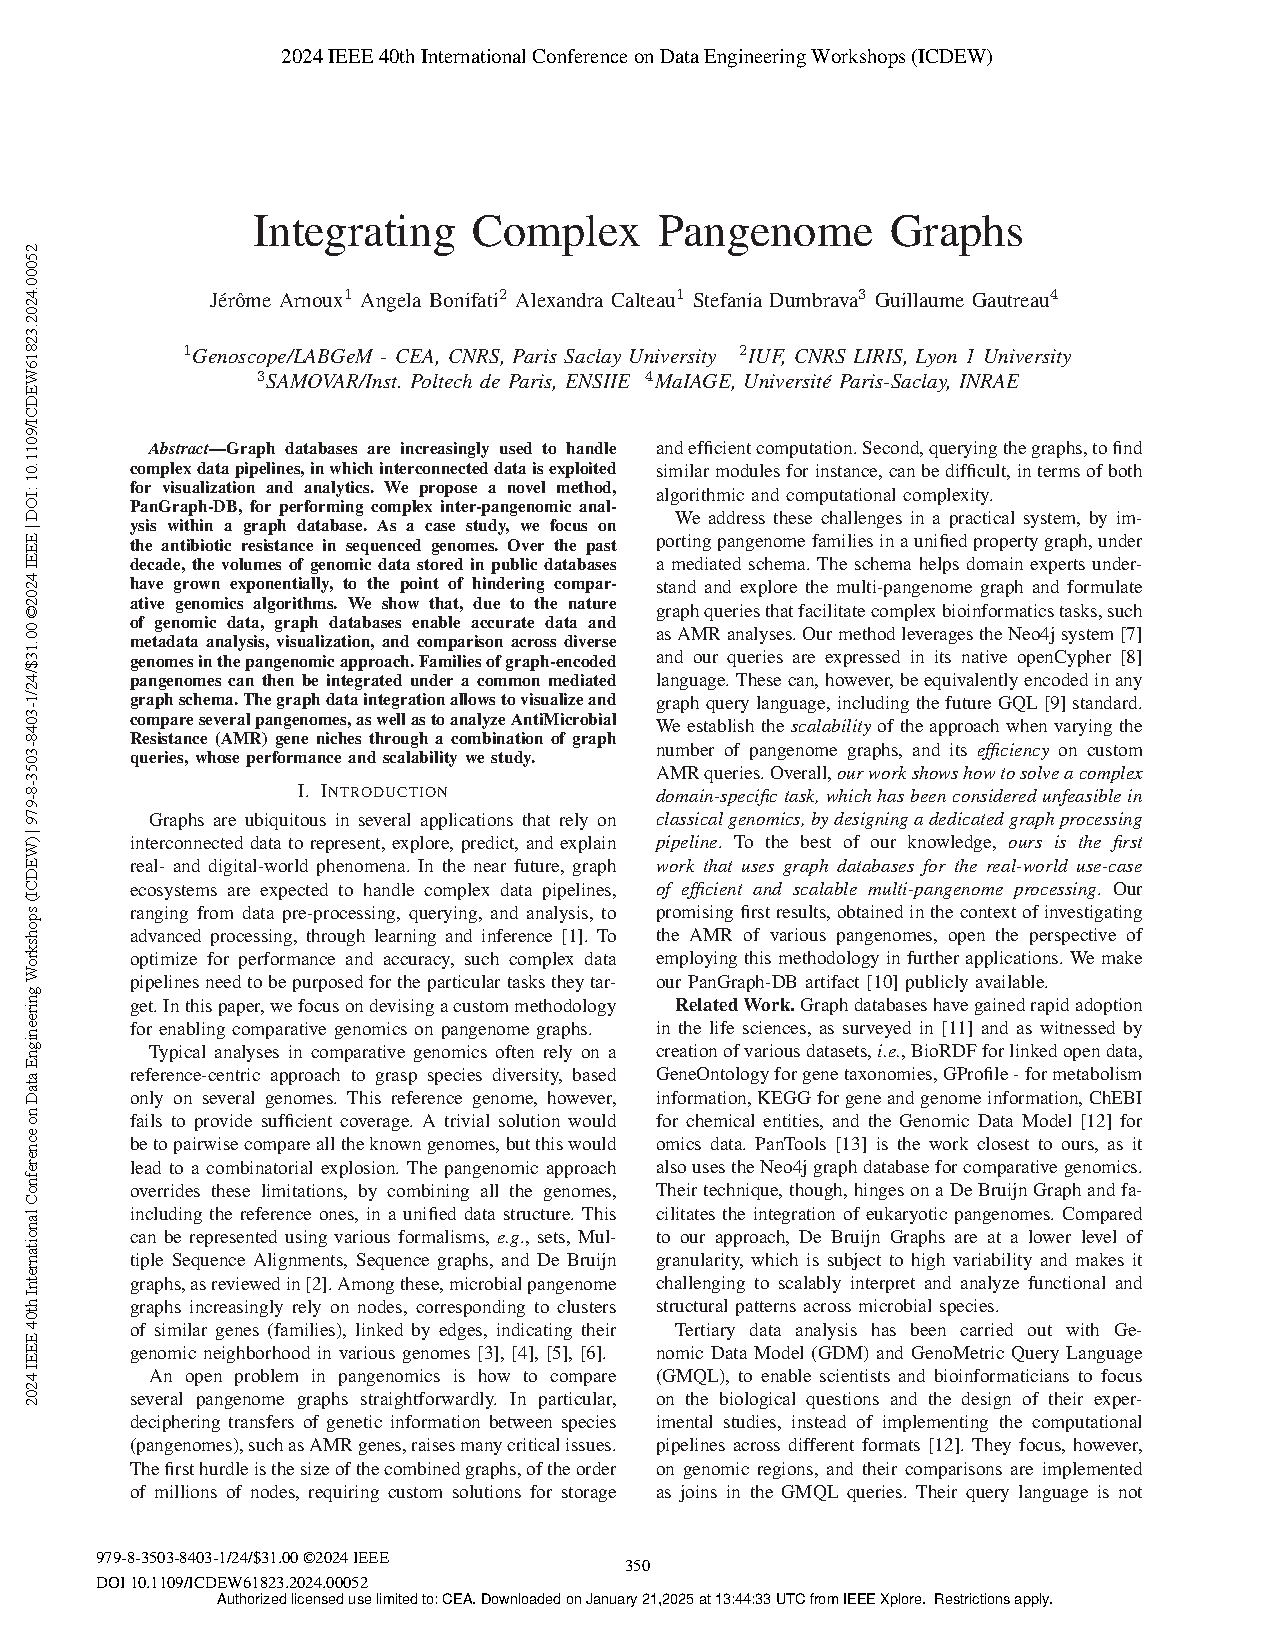
\includepdf[pages=-]{GraphDataBase/Integrating_Complex_Pangenome_Graphs.pdf}

\chapter{Conclusion et perspectives}

Notre \textit{proof of concept} sur l'intégration et l'analyse de pangénomes dans des bases de données orientées graphe, ouvre la voie à de nouvelles méthodes de stockage, d’analyse et de visualisation de vastes ensembles de génomes et de pangénomes. Nous avons conçu un schéma de base de données ainsi qu’un workflow d’analyse générique, pouvant être adaptés à d'autres modèles de pangénomes. Nos tests montrent que notre approche permet des temps de réponse très rapides (de l’ordre de la milliseconde) aussi bien pour des requêtes simples que pour des analyses complexes. Bien que notre POC soit une réussite, plusieurs améliorations sont nécessaires pour en faire une véritable base de données opérationnelle dédiée à l’analyse et à la distribution des pangénomes.

Pour intégrer les pangénomes dans la base de données, j'ai développé un script Python utilisant \textbf{PPanGGOLiN} et \textbf{PANORAMA} afin d’extraire et de préparer les données. L’intégration dans Neo4j s’est appuyée sur des packages tiers, non optimisés pour nos données, entraînant des temps d’intégration relativement longs. Récemment, Neo4j a publié un package officiel, plus flexible et optimisé pour la communication avec la base. Les premiers tests, que j'ai menés, indiquent qu’il permettrait une réduction significative des temps d’intégration, ce qui constitue une piste prometteuse pour améliorer l'efficacité globale du système.

Lors d’un second hackathon D4GEN en 2023, l’intégration de \textbf{méthodes de machine learning} a été explorée dans notre workflow d’analyse. Neo4j propose plusieurs packages dédiés à l’application du ML directement sur la base de données. Nous avons testé différentes approches pour identifier des structures et des chemins pertinents dans le graphe de pangénome, mais aucun résultat probant n’a émergé.
Cependant, cette première tentative nous a permis de repenser le schéma de la base de données et d'imaginer de \textbf{nouvelles métadonnées} à intégrer pour des analyses futures.

Pour construire la BD Neo4J, j'ai développé un script permettant de charger les pangénomes dans une base de données locale. Ce script avait d'abord été intégré à PANORAMA, pour sa capacité à lire plusieurs pangénomes. Toutefois, nous avons finalement choisi de développer un script indépendant, plus facile à maintenir. Ce script offre plusieurs avantages : intégration simplifiée des pangénomes dans la base, lancement automatique des analyses, indépendance vis-à-vis de l’interface Neo4j.
L’objectif étant de rendre l’ensemble du processus plus accessible et automatisé, afin que chacun puisse créer une instance propre de base de données de pangénomes.

Le \textbf{LABGeM} développe une base de données de pangénomes générés par PPanGGOLiN, \textbf{PanGBank}. Ce projet repose sur une architecture de BD relationnelle \textbf{SQL}, contenant les fichiers \textbf{HDF5} pour chaque espèce et des résultats d’analyse accessibles en ligne.
Une intégration avec notre POC pourrait offrir plusieurs avantages :
\begin{itemize}
    \item Une \textbf{nouvelle manière d’organiser et de visualiser les pangénomes}
    \item La possibilité d’\textbf{effectuer des analyses complexes directement sur la base de données}
    \item Une meilleure interconnexion entre les données et les outils d’exploration
\end{itemize}
En combinant ces approches, nous pourrions développer un système de gestion des pangénomes plus robuste, interactif et performant.


\end{document}